\chapter{Introducci\'{o}n}
\textit{Staphylococcus aureus} es una bacteria pat\'{o}gena Gram positiva que causa enfermedades infecciosas. De acuerdo a Kobayashi et al. \cite{Kobayashi2015PathogenesisAbscesses}, la bacteria es un colonizador com\'{u}n de la piel y del aparato respiratorio y act\'{u}a como un pat\'{o}geno oportunista que puede causar infecciones nicosomiales (intrahospitalarias) en el sistema respiratorio, en los tejidos blandos y en el torrente sangu\'ineo \cite{HarpavatS.NissimS.LipppincottsMicrocards:MicrobiologyFlashCards2012.}. Incluso puede causar infecciones en las junturas de las pr\'otesis formando biopel\'iculas \cite{Meylan2018}.\\

%En la figura \ref{fig:sta} se muestra una microfotograf\'ia de \textit{Staphylococcus aureus} resistente a antibi\'oticos.\\

%\begin{figure}[h]
%\begin{center}
 % 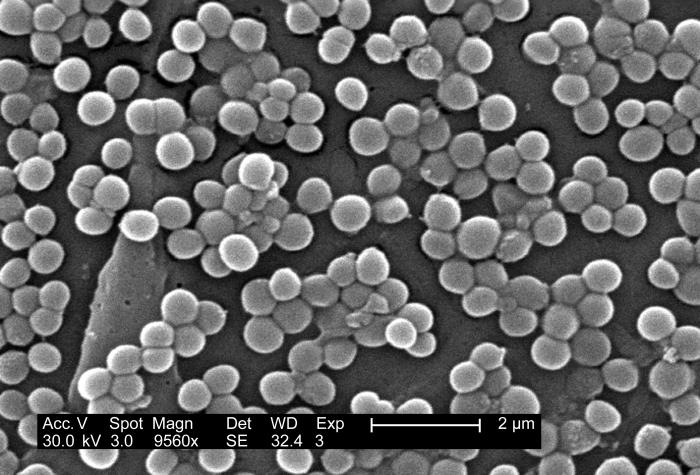
\includegraphics[scale=0.3]{saureus.jpg}
  %\caption{Imagen  de \textit{Staphylococcus aureus} obtenida con un microscopio electr\'onico de barrido (SEM). Tomado de \cite{HaneyCar2005PublicAureus}.}
  %\label{fig:sta}
%\end{center}
%\end{figure}

Desde el descubrimiento de \textit{Staphylococcus aureus} como causante de una infecci\'on a una herida en 1881 \cite{Orent2006AMagazine} se ha investigado su presencia en otras infecciones y se han utilizado antibi\'oticos como la penicilina, la meticilina y la vancomicina para controlar estas infecciones   \cite{HarpavatS.NissimS.LipppincottsMicrocards:MicrobiologyFlashCards2012.}. No obstante, \textit{Staphylococcus aureus} ha desarrollado resistencia a algunos de estos antibi\'oticos,  de ah\'{i} que surja la necesidad de buscar nuevos antibi\'oticos o incluso mol\'{e}culas con un mecanismo de acci\'{o}n diferente. Una posible familia de mol\'{e}culas que podr\'{i}an actuar como alternativas ser\'{i}an los p\'{e}ptidos antimicrobianos. Estas mol\'{e}culas son polip\'{e}ptidos cortos de alrededor de 1000 $k$D que se adhieren selectivamente a membranas bacterianas, generando poros y compremetiendo los gradientes electroqu\'{i}micos esenciales para su funcionamiento. \\

De acuerdo a Perez-Lopez et al. \cite{Perez-Lopez2019VariationsProperties} y a Nagendra et al.  \cite{Nagendra2011} se ha encontrado que la bacteria modula la composici\'{o}n de su membrana plasm\'{a}tica frente a cambios en el medio. Esta modulaci\'{o}n afecta las propiedades biof\'{i}sicas de su membrana, es decir propiedades fisicoqu\'{i}micas como la permeabilidad, la estructura y las propiedades mec\'{a}nicas. El cambio de estas propiedades es un factor que mejora la tolerancia de la bacteria a la acci\'{o}n de p\'{e}ptidos antimicrobiales. Variaciones en las propiedades mec\'{a}nicas que resultan al generarse cambios en la composici\'{o}n lip\'{i}dica de la bacteria impiden la penetraci\'{o}n de estos p\'{e}ptidos en la membrana e inhiben la formacion de poros. Debido a esto, las propiedades biof\'{i}sicas de la membrana se convierten en objeto de estudio y adem\'{a}s son determinantes en la b\'{u}squeda de nuevas mol\'{e}culas dirigidas a la membrana (mol\'{e}culas blanco) que combatan la bacteria. \\

\textit{Staphylococcus aureus}\footnote{\textit{Staphylococcus aureus} es una bacteria Gram positiva, lo cual implica que solo tiene una membrana celular.  La membrana es una bicapa lip\'{i}dica de alrededor de 4 nm de grosor, compuesta principalmente de fosfol\'{i}pidos como diacil fosfatidil-gliceroles, cardiolipinas y carotenoides como la estafiloxantina. La membrana es impermeable a iones como protones, sodio, potasio y cloro, lo que le permite mantener gradientes electroquim\'{i}cos que son usados para generaci\'{o}n de energ\'{i}a y senalizaci\'{o}n. Esta membrana esta recubierta de una pared externa de p\'{e}ptidoglicanos los cuales proveen estructura mec\'{a}nica y protegen la integridad de la membrana. Las membranas se explican en mas detalle en la subsecci\'{o}n \ref{ss:mem}}. Algunos estudios se han enfocado en c\'{o}mo la composici\'{o}n de la bicapa lip\'{i}dica interna afecta sus propiedades biof\'{i}sicas con base en cambios en la concentraci\'{o}n de ciertos l\'{i}pidos como la cardiolipina \cite{Hernandez-Villa1BiophysicalPeptides} y de carotenoides como la estafiloxantina \cite{Melendez-Delgado2018StudyingBilayers}, \cite{Perez-Lopez2019VariationsProperties}, \cite{Nagendra2011}. Recientemente, nuestro grupo, se ha enfocado en estudiar computacionalmente y experimentalmente propiedades mec\'{a}nicas como la rigidez de la membrana, la orientaci\'{o}n de fosfolip\'{i}dos y carotenoides, el \'{a}rea por l\'{i}pido, la difusi\'{o}n y el par\'{a}metro de orden del deuterio de las cadenas aciles para diferentes membranas modelo.\\

En los experimentos realizados por Perez-Lopez et al. \cite{Perez-Lopez2019VariationsProperties} y Nagendra et al.  \cite{Nagendra2011} se ha mostrado que cambios en el contenido de carotenoides en las membranas, en diferentes etapas de crecimiento \textit{Staphylococcus aureus}, y en membranas modelo compuestas por algunos l\'{i}pidos mayoritarios de la bacteria, resultan en cambios en la rigidez. Se ha demostrado que este cambio en la rigidez afecta la resistencia de la membrana a diferentes p\'{e}ptidos antimicrobiales. Sin embargo, es necesario mirar a nivel molecular la influencia local que tienen los carotenoides en la membrana para entender con mas precisi\'{o}n como la presencia de estas mol\'{e}culas puede influir en las propiedades mec\'{a}nicas. Debido a su resoluci\'{o}n, los experimentos realizados no permiten vislumbrar diferentes propiedades moleculares que puedan explicar este fen\'{o}meno. Alternativamente, las simulaciones de din\'{a}mica molecular (MD por sus siglas en ingl\'{e}s) si permiten hacer este acercamiento. La MD se ha convertido en una herramienta excelente para estudiar membranas biol\'{o}gicas \cite{Marrink2019ComputationalMembranes}. Este m\'{e}todo monitorea la evoluci\'{o}n espacio-temporal de sistemas biol\'{o}gicos a una escala at\'{o}mica y asi permite determinar informaci\'{o}n estructural, (termo)din\'{a}mica y energ\'{e}tica de membranas, que complementa y expande las t\'{e}cnicas experimentales. \\

Entre las propiedades que se pueden estudiar en detalle a trav\'{e}s de simulaciones est\'{a}n la ubicaci\'{o}n relativa de los carotenoides con respecto a los otros l\'{i}pidos y la orientaci\'{o}n. Adicionalmente se pueden estudiar las interacciones que presenta exclusivamente el carotenoide estafiloxantina con los l\'{i}pidos vecinos y los efectos que tiene la presencia de estafiloxantina en la orientaci\'{o}n y organizacion de los l\'{i}pidos vecinos. Estos detalles moleculares influyen en los cambios de la rigidez de la membrana de \textit{Staphylococcus aureus} y pueden alterar la susceptibilidad de la membrana a la presencia de peptidos antimicrobiales.\\

Para estudiar la ubicaci\'{o}n, las interacciones con otros l\'{i}pidos, el \'{a}rea por l\'{i}pido y el par\'{a}metro de orden del deuterio  sobre la estafiloxantina, en nuestro grupo se ha realizado un estudio computacional preeliminar mediante las simulaciones por din\'{a}mica molecular  implementadas en CHARMM \cite{Melendez-Delgado2018StudyingBilayers}. Estas simulaciones requieren introducir par\'{a}metros relacionados con los campos de fuerza y con la geometr\'{i}a de la estafiloxantina, los cuales deben ser cuidadosamente seleccionados para que las simulaciones por din\'{a}mica molecular reflejen el comportamiento f\'{i}sico de la mol\'{e}cula.\\

En una aproximaci\'{o}n inicial, Mel\'{e}ndez et al. \cite{Melendez-Delgado2018StudyingBilayers} utilizaron el protocolo implementado en CHARMM-GUI \cite{Brooks2009} para determinar los par\'{a}metros del campo de fuerza de estafiloxantina. Algunos de los par\'{a}metros obtenidos a trav\'{e}s de este procedimiento no se optimizaron completamente, en particular los par\'{a}metros alrededor del grupo carbonil presente en la cadena diaponeurosporenoica de la estafiloxantina. Este grupo inicialmente se parametriz\'{o} sin considerar la presencia del ox\'{i}geno el cual debe influir en las constantes de torsi\'{o}n de los \'{a}ngulos dihedros adyacentes al grupo carbonil. Debido al vac\'{i}o existente en los par\'{a}metros de la mol\'{e}cula, surgi\'{o} la necesidad de optimizar la parametrizaci\'{o}n completa de toda la cadena conjugada por otros m\'{e}todos para as\'{i} tener certeza sobre los resultados preliminares y para poder confiar en la interpretaci\'{o}n de los resultados.\\

Por esto, durante la realizaci\'{o}n del presente documento, el integrante David R. Figueroa y el director Gian P. Miscione pertenecientes al grupo COBO del Departamento de Qu\'{i}mica de la Universidad de los Andes realizaron una optimizaci\'{o}n de los par\'{a}metros del potencial dih\'{e}drico para dicho carbonil mediante m\'{e}todos mec\'{a}nico-cu\'{a}nticos, de estos par\'{a}metros se obtuvo una mol\'{e}cula con la misma forma del potencial hallado inicialmente con CHARMM-GUI pero con una barrera de potencial m\'{a}s alta, por lo cual de estafiloxantina m\'{a}s r\'{i}gida. \\

Una vez obtenidos estos par\'{a}metros se realizaron 10 simulaciones por din\'{a}mica molecular para diferentes composiciones. Los l\'{i}pidos modelo que se seleccionaron son 1,2-dimiristoil-sn-glicero-3-fosfocolina (DMPG) y 1,2-dipalmitoil-sn-glicero-3-fosfocolina (DPPG). Cada uno de estos lipidos contiene dos cadenas aciles saturadas id\'{e}nticas. En el caso de DMPG las cadenas son de 14 carbones y en el caso de DPPG las cadenas son de 16 carbones. Esta diferencia nos permite estudiar como el grosor de la membrana influye en la organizaci\'{o}n de estafiloxantina. Se escogen l\'{i}pidos con cabezas polares tipo fosfoglicerol debido a que estas cabezas polares son prevalentes en las membranas de \textit{Staphylococcus aureus}, \cite{Sohlenkamp2015BacterialPathways}. Las simulaciones de los sistemas puros de DMPG y DPPG se comparan con sistemas que tienen diferentes contenidos de estafiloxantina. Se estudiaron las siguientes concentraciones para ver el efecto de el carotenoide sobre las membranas puras: 1 STX:128 DMPG, 1 STX:128 DPPG, 15\% mol de STX en DMPG y 15\% mol STX en DPPG. Los sistemas estudiados pueden resumirse en la siguiente tabla:\\

\begin{table}[h]
    \centering
    \begin{tabular}{|c|c|}\hline
        \textbf{L\'{i}pidos} & \textbf{Composici\'{o}n} \\\hline
        DMPG &128 DMPG \\
        DPPG &128 DPPG \\
        Estafiloxantina y DMPG &1 STX:128 DMPG \\
        Estafiloxantina y DPPG  &1 STX:128 DPPG\\
         15\% Estafiloxantina y DMPG &64 STX: 362 DMPG\\
         15\% Estafiloxantina y DPPG&64 STX: 362 DPPG\\
         15\% Estafiloxantina r\'{i}gida con y DMPG&64 STX: 362 DMPG\\
         15\% Estafiloxantina r\'{i}gida y DPPG&64 STX: 362 DMPG\\ \hline
    \end{tabular}
    \caption{Los diez sistemas utilizados para representar la membrana bacteriana de \textit{Staphylococcus aureus} est\'{a}n compuestos por DMPG, DPPG o estafiloxantina. Estafiloxantina \textit{r\'{i}gida} es una convenci\'{o}n hecha para nombrar los par\'{a}metros obtenidos por D.R. Figueroa y G.P. Miscione del grupo COBO.}
    \label{tab:my_label}
\end{table}

Una vez obtenidas las trayectorias de las simulaciones se han calculado y analizado de forma global la orientaci\'{o}n de la estafiloxantina, el \'{a}rea por l\'{i}pido, el espesor de la membrana y el nivel de interdigitaci\'{o}n tanto de los fosfol\'{i}pidos como de la estafiloxantina. Estas mediciones fueron llevadas a cabo por D. R. Figueroa del grupo COBO. En este documento de tesis se reporta el efecto de la presencia de estafiloxantina en el coeficiente de difusi\'{o}n de la membrana, y el perfil de estr\'{e}s a lo largo de la coordenada z. Con el fin de comparar con las mediciones globales de espesor y area por l\'{i}pido calculados por D. R. Figueroa, en esta tesis se calcularon estas mismas propiedades pero a nivel local. Se hace una comparaci\'{o}n con estas mediciones para determinar de manera m\'{a}s robusta estos par\'{a}metros con el fin de reportarlos de manera fiable en una futura publicaci\'{o}n.
%%Gracias a estos par\'{a}metros fue posible la realizaci\'{o}n de las simulaciones de algunos de los sistemas presentes.